\newpage
\section{Vatnets gang gjennom anlegget}
\begin{figure}[htbp]
    \centering
    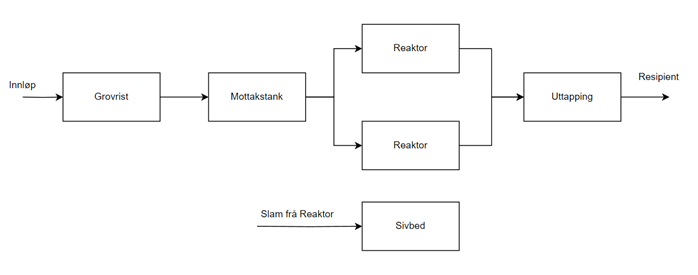
\includegraphics[width=1\textwidth]{Figurar/VannetsGangGjennomAnlegget.png}
    \caption{Vatnets gang gjennom annlegget}\label{fig:Vatnets Gang}
\end{figure}

Ved normal drift kjem avløpsvatnet inn til anlegget via innløpsrøyret til ein forbehandlingseining, for dette anlegget ein Hydropress – «Huber rotomat RO9» innløpsrist med ristgodsvasker og presse.
Denne risten held tilbake uorganisk materiale som Q-tips, plast sanitetsbind osv. Dette er material som eit ikkje ønsker å ha med vidare i prosessen. 
Framandlegeme i avløpsvatnet kan føre til skader på pumper, ventilar og andre prosesskomponentar. Forbehandlingsdelet er utforma for å fjerne minst mogleg organisk materiale. Dette samsvarer med verkemåte på biologisk reinsing.

Frå rista renner vatnet med sjølvfall til mottakstanken. Hovudfunksjonen til denne tanken i tillegg til at den fungerer som pumpetank er å utjamne større periodiske tilstrøymingsmenger og fungera som oppsamlingstank ved straumbrot. 
Frå mottakstanken pumpes vatnet vidare til reaktorane. 

Innpumping skjer til den reaktoren "som står for tur", dvs. den har drenert av reinsa vann og er i riktig fase (innpumpingsfase). 
Når vatnet er pumpa opp til en reaktor, føregår all reinsing i den same tanken. Vatnet blir dermed ikkje flytta frå tank til tank.

Dersom ingen av tankane er i innpumpingsfase blir vatnet lagra i mottakstanken, inntil en av reaktorane har avslutta sin syklus.

Etter biologisk/kjemisk reinsing i en av reaktortankane blir det reinsa avlaupsvatnet drenert via utlaupsrøyret til elva Gaula. 
På utløpsrøyret er det eit prøvetakingspunkt. 





    